%!TEX root = ../template.tex
%%%%%%%%%%%%%%%%%%%%%%%%%%%%%%%%%%%%%%%%%%%%%%%%%%%%%%%%%%%%%%%%%%%
%% chapter1.tex
%% NOVA thesis document file
%%
%% Chapter with introduction
%%%%%%%%%%%%%%%%%%%%%%%%%%%%%%%%%%%%%%%%%%%%%%%%%%%%%%%%%%%%%%%%%%%

% NOTE: Cite \cite{novathesis-manual} somewhere, in your thesis/dissertation with “\verb!\cite{novathesis-manual}!”, any place you think it makes sense.  If you cite it this way, the correct entry will be added automatically to your bibliography (there no need to add it to your BibTeX file);

\typeout{NT FILE chapter1.tex}

\chapter{Introduction}\label{cha:introduction}

\prependtographicspath{{Chapters/Figures/Covers/phd/}{Chapters/Figures/Covers/msc/}}

% epigraph configuration
% \epigraphfontsize{\small\itshape}
% \setlength\epigraphwidth{12.5cm}
% \setlength\epigraphrule{0pt}

\begin{figure}[H]
  \centering
	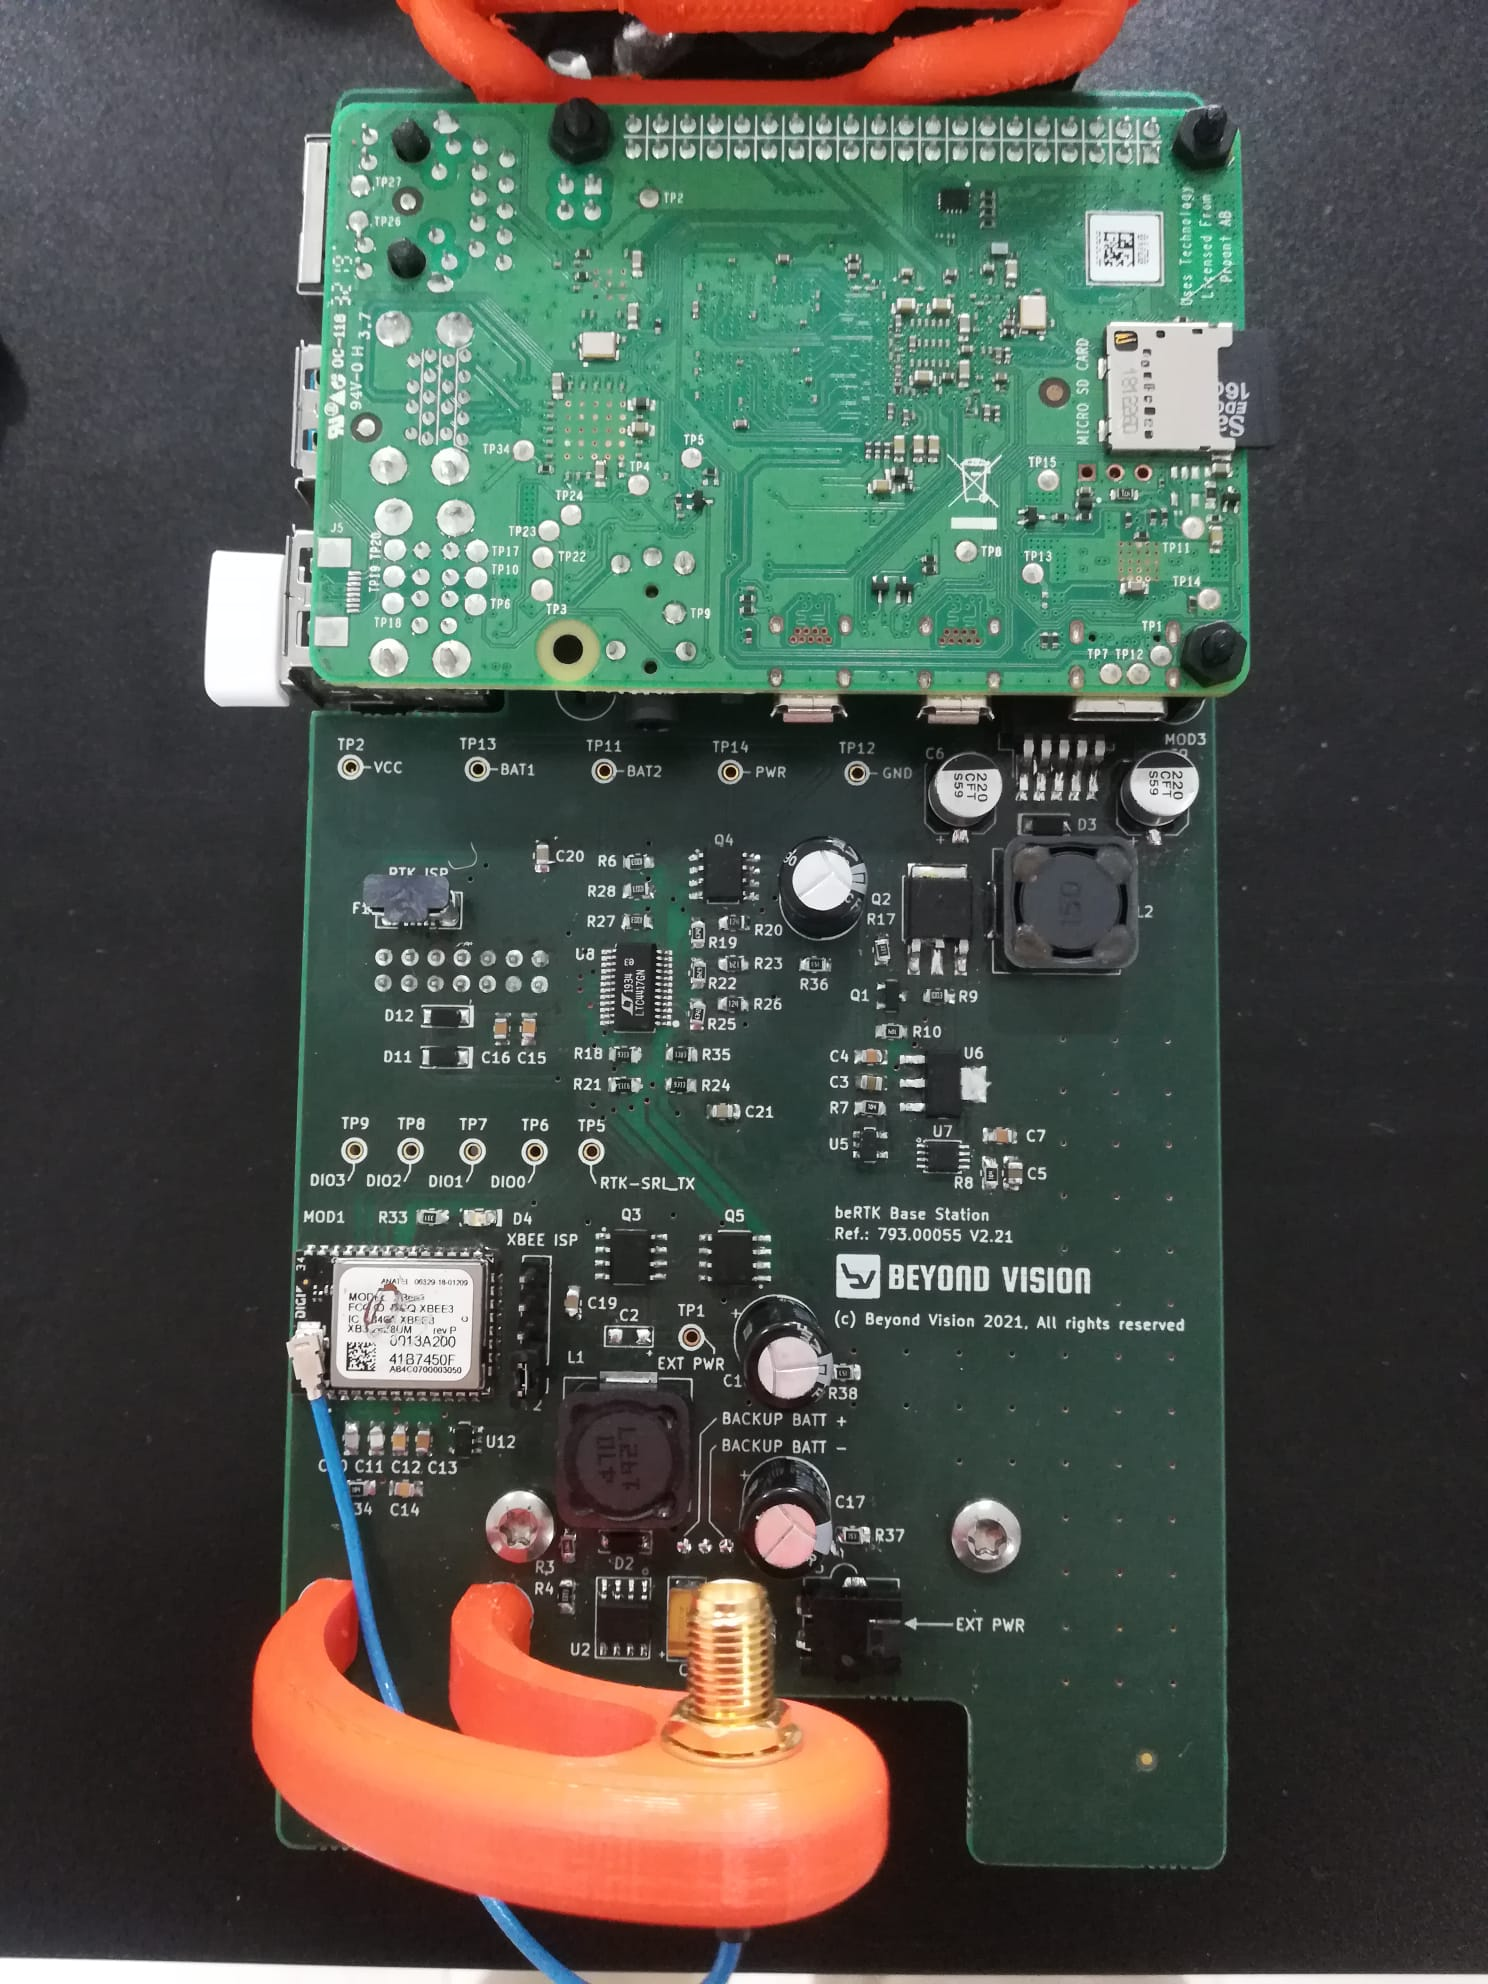
\includegraphics[width=0.5\textwidth, keepaspectratio]{Chapters/Figures/Intro/old_BS.jpeg}
	\caption{Old base station.}
	\label{fig:old_BS}
\end{figure}

% \epigraph{
%   This work is licensed under the \href{LaTeX project public license}{\LaTeX\ Project Public License v1.3c}.
%   To view a copy of this license, visit \url{LaTeX project public license}.
% }

This is Figure \ref{fig:old_BS}. It shows the current \gls{base_station}.

\section{Subsection 1.1}\label{sub:sub1_1}

\section{Subsection 1.2}\label{sec:sub1_2}

\section{Subsection 1.3}\label{sec:sub1_3}

The template provides an \emph{easy-to-use} setting for you to write your thesis/dissertation in \LaTeX:

\subsection{Using Overleaf}\label{sub:using_overleaf}

If you do not have an account in \href{https://www.overleaf.com?r=f5160636&rm=d&rs=b}{Overleaf}, you must \href{https://www.overleaf.com?r=f5160636&rm=d&rs=b}{create one first}.

Once you have an account, please access the \glsxtrlong{novathesis} in \href{https://www.overleaf.com/latex/templates/new-university-of-lisbon-universidade-nova-de-lisboa-slash-unl-thesis-template/fwbztcrptjmg}{Overleaf} and select the green button \emph{Open as Template}.

\emph{Please note that the version currently available in Overleaf (v4.1.3) is outdated. A new version will be submitted to Overleaf soon.}

\subsection{Using a Local \LaTeX\ Installation}
\label{sub:using_local_latex}

\begin{wrapfigure}{r}{0.5\linewidth}
\vspace*{-15ex}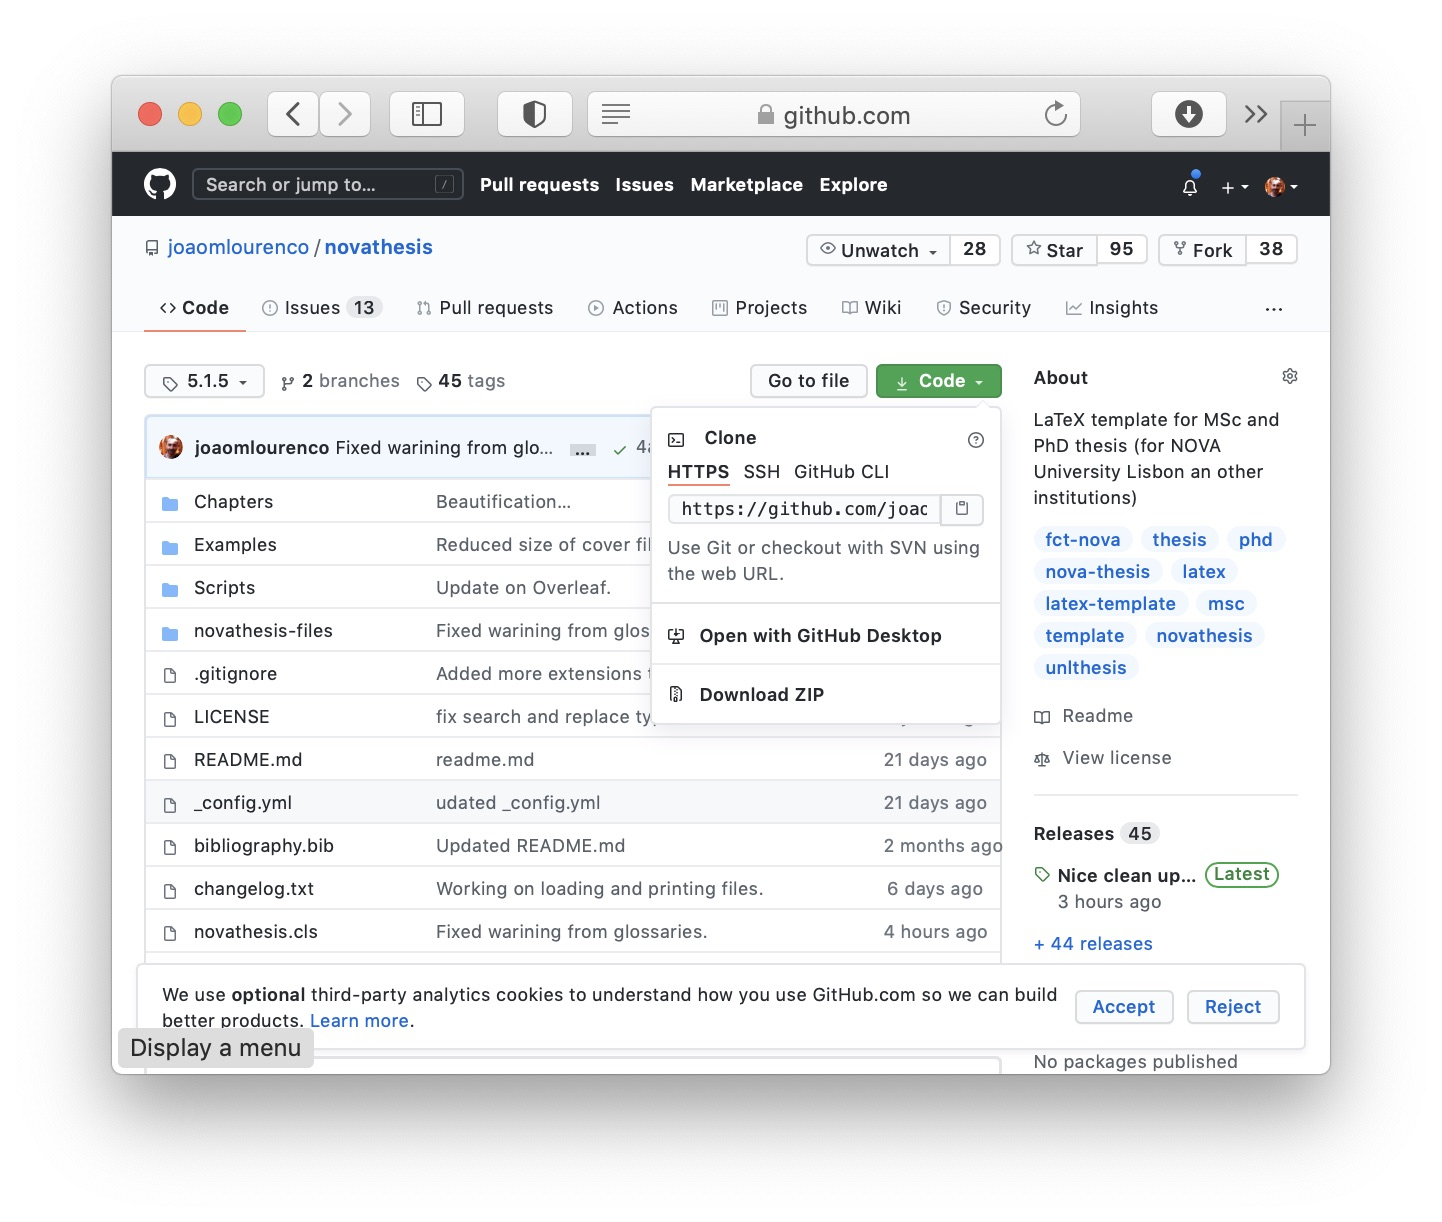
\includegraphics[width=\linewidth]{github}%
\end{wrapfigure}

Just access the \glsxtrlong{novathesis} in \href{https://github.com/joaomlourenco/novathesis}{GitHub}, select the green button \emph{Code} and then \emph{download} (or \emph{clone}) the template.  You will always get the latest version of the template (currently v5.1.8).

\section{Getting Help}
\label{sec:getting_help}

\subsection{Google}
\label{sub:group_google}

Remember, when looking for hints or help, \emph{\href{google.com}{Google} is your best friend}!   And if you prefix your Google query with “\emph{LaTeX}”, your fist link will most probably direct you to \texttt{tex.stackexchange.com}.

\subsection{Group Support}
\label{sub:group_support}

To get directed help on the \glsxtrlong{novathesis} please join:
\begin{itemize}
  \item the \href{https://www.facebook.com/groups/novathesis}{NOVAtheis Facebook group}, or
  \item the \href{https://groups.google.com/forum/#!forum/novathesis}{NOVAthesis Google group}.
\end{itemize}

There were huge changes from version 4.x.y to version 5.a.b so, please, \textbf{always} state the version number you are using when asking for help.

\subsection{Reporting Problems}
\label{sub:reporting_problems}

If you just need some help, see above \ref{sub:group_google} and \ref{sub:group_support} \Autoref{sub:group_google} and \Autoref{sub:group_support}.

If you believe \emph{you found a bug} or if \emph{you need some improvement} in the template, please \href{https://github.com/joaomlourenco/novathesis/issues}{fill an issue in github} at \url{https://github.com/joaomlourenco/novathesis/issues}.

\section{Donations}
\label{sec:donations}

This template is the result of hundreds (yes! \emph{may hundreds}!) of hours of work from the \href{https://docentes.fct.unl.pt/joao-lourenco}{main developer}.  If you think this template really made you life easier while writing your thesis, please consider \href{https://paypal.me/novathesis}{\textbf{making a donation}}. We will keep a list thanking to all the identified donors that identify themselves in the “\emph{Add special instructions to the seller}” box.

\subsubsection*{Donors 2020}
\label{ssub:donors_2020}

\begin{inparaitem}[]
  \item João Carvalho,
  \item David Romão,
  \item DisplayersereStream, and
  \item António Estêvão.
\end{inparaitem}

\subsubsection*{Donors 2019}
\label{ssub:donors_2019}

\begin{inparaitem}[]
  \item Jorge Barreto and
  \item Raissa Almeida.
\end{inparaitem}

\section{Disclaimer}
\label{sec:disclaimer}

Although this template is endorsed by the FCT-NOVA and even \href{https://www.fct.unl.pt/estudante/informacao-academica}{linked from its web site}, this is still not an official template.
%
This template exists to make your life easier and we do our best to make the \gls{novathesis} template compliant to the supported Schools' regulations, but in the end of the line you and only you are accountable for both the look and the contents of the document you submit as your thesis/dissertation.

% \printbibliography[heading=subbibliography, segment=\therefsegment, title={\bibname\ for chapter~\thechapter}]
